\documentclass[11pt,letterpaper]{article}
\usepackage[lmargin=1in,rmargin=1in,tmargin=1in,bmargin=1in]{geometry}
\usepackage{../style/homework}
\setbool{quotetype}{true} % True: Side; False: Under
\setbool{hideans}{false} % Student: True; Instructor: False

% -------------------
% Content
% -------------------
\begin{document}

\homework{19: Due 04/22}{I was so unpopular in high school, the crossing guard used to lure me into traffic.}{Annie Edison, Community}

% Problem 1
\problem{10} Consider the function $z= -65x_1 + 5x_2$ on the region $\mathcal{R}$ shown below. Does $z$ have a maximum or minimum value on $\mathcal{R}$? Explain. If the function has a maximum or minimum value on $\mathcal{R}$, find the maximum and minimum value. 
	\[
	\fbox{
	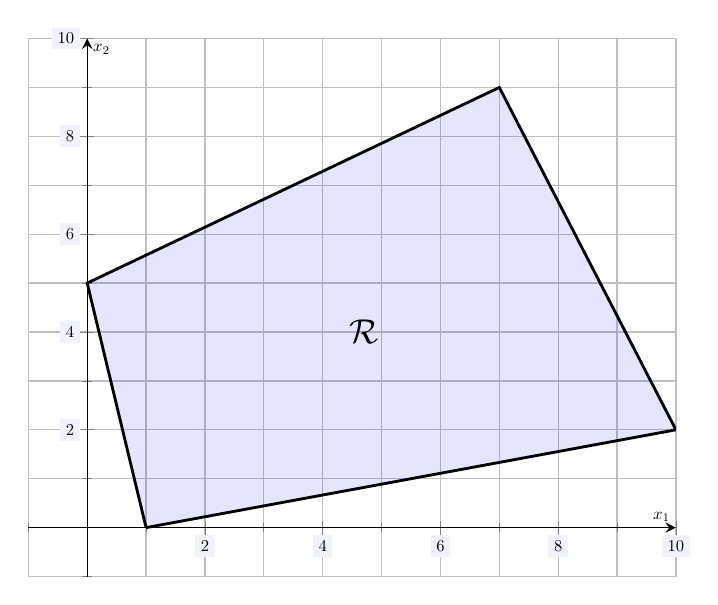
\begin{tikzpicture}[scale=1.2,every node/.style={scale=0.5}]
	\begin{axis}[
	grid=both,
	axis lines=middle,
	ticklabel style={fill=blue!5!white},
	xmin= -1, xmax=10,
	ymin= -1, ymax=10,
	xtick={0,2,4,6,8,10},
	ytick={0,2,4,6,8,10},
	minor tick = {-1,0,1,...,10},
	xlabel=\(x_1\),ylabel=\(x_2\),
	]
	\draw[line width=0.01cm,fill= blue,opacity=0.1] (1,0) -- (0,5) -- (7,9) -- (10,2) -- (1,0);
	\draw[line width=0.03cm] (1,0) -- (0,5) -- (7,9) -- (10,2) -- (1,0);
	\node at (4.7,4.0) {\huge$\mathcal{R}$};
	\end{axis}
	\end{tikzpicture}
	}
	\] \pspace

\sol The function $z= -65x_1 + 5x_2$ is a linear function. The region $\mathcal{R}$ is a nonempty, bounded region. Therefore, by the Fundamental Theorem of Linear Programming, there exists a maximum and minimum for $z$ on $\mathcal{R}$ and they occur at a corner point for $\mathcal{R}$. We need only examine $z$ at these points: \par
	\begin{table}[h]
	\centering
	\begin{tabular}{cl}
	Corner Point & $z(x_1, x_2)$ \\ \hline
	$(1, 0)$ & $z(1, 0)= -65(1) + 5(0)= -65 + 0= -65$ \\
	$(0, 5)$ & $z(0, 5)= -65(0) + 5(5)= 0 + 25= 25$ \\
	$(7, 9)$ & $z(7, 9)= -65(7) + 5(9)= -455 + 45= -410$ \\
	$(10, 2)$ & $z(10, 2)= -65(10) + 5(2)= -650 + 10= -640$
	\end{tabular}
	\end{table} \par
Therefore, the maximum value for $z$ is $25$ and occurs at $(0, 5)$ and the minimum value for $z$ is $-640$ and occurs at $(10, 2)$. 



\newpage



% Problem 2
\problem{10} Consider the function $z= 6x_1 + 11x_2$ on the region $\mathcal{R}$ shown below. Does $z$ have a maximum or minimum value on $\mathcal{R}$? Explain. If the function has a maximum or minimum value on $\mathcal{R}$, find the maximum and minimum value. 
	\[
	\fbox{
	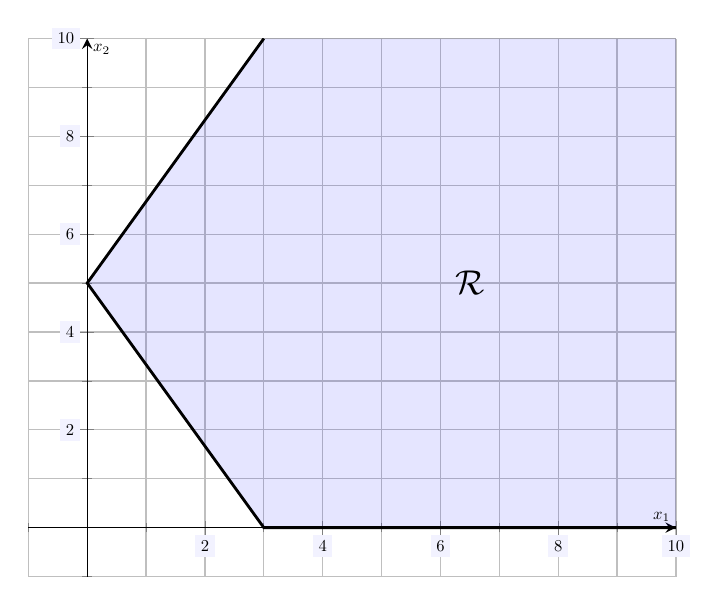
\begin{tikzpicture}[scale=1.2,every node/.style={scale=0.5}]
	\begin{axis}[
	grid=both,
	axis lines=middle,
	ticklabel style={fill=blue!5!white},
	xmin= -1, xmax=10,
	ymin= -1, ymax=10,
	xtick={0,2,4,6,8,10},
	ytick={0,2,4,6,8,10},
	minor tick = {-1,0,1,...,10},
	xlabel=\(x_1\),ylabel=\(x_2\),
	]
	
	\draw[line width=0.01cm,fill= blue,opacity=0.1] (10,0) -- (3,0) -- (0,5) -- (3,10) -- (10,10) -- (10,0);	
	\draw[line width=0.03cm] (10,0) -- (3,0) -- (0,5) -- (3,10);
	\node at (6.5,5) {\huge$\mathcal{R}$};
	\end{axis}
	\end{tikzpicture}
	}
	\] \pspace

\sol The function $z= 6x_1 + 11x_2$ is linear. The region $\mathcal{R}$ is nonempty. However, the region $\mathcal{R}$ is not bounded, i.e. it is unbounded. Therefore, the Fundamental Theorem of Linear Programming does not apply. The function $z$ may have a maximum, a minimum, both, or neither. Observe that increasing $x_1$ increases $z$. Furthermore, increasing $x_2$ also increases $z$. Increasing $x_1$ and $x_2$ moves the point $(x_1, x_2)$ to the right and up, respectively. Because there is no limit to how much one can move upwards and to the right in $\mathcal{R}$, there is no limit to how large $z$ can become. Therefore, $z$ has no maximum. Correspondingly, moving downwards and to the left decreases $z$. One can only move so far in these directions and stay in $\mathcal{R}$. Therefore, there is a minimum value for $z$ and it must occur at a corner point for $\mathcal{R}$. We simply examine $z$ at these points. \par
	\begin{table}[h]
	\centering
	\begin{tabular}{cl}
	Corner Point & $z(x_1, x_2)$ \\ \hline
	$(3, 0)$ & $z(3, 0)= 6(3) + 11(0)= 18 + 0= 18$ \\
	$(0, 5)$ & $z(0 ,5)= 6(0) + 11(5)= 0 + 55= 55$
	\end{tabular}
	\end{table} \par
Therefore, the minimum value for $z$ is $18$ and occurs at the point $(3, 0)$. 



\newpage



% Problem 3
\problem{10} Consider the function $z= x_1 + 7x_2$ on the region $\mathcal{R}$ shown below. Does $z$ have a maximum or minimum value on $\mathcal{R}$? Explain. If the function has a maximum or minimum value on $\mathcal{R}$, find the maximum and minimum value. 
	\[
	\fbox{
	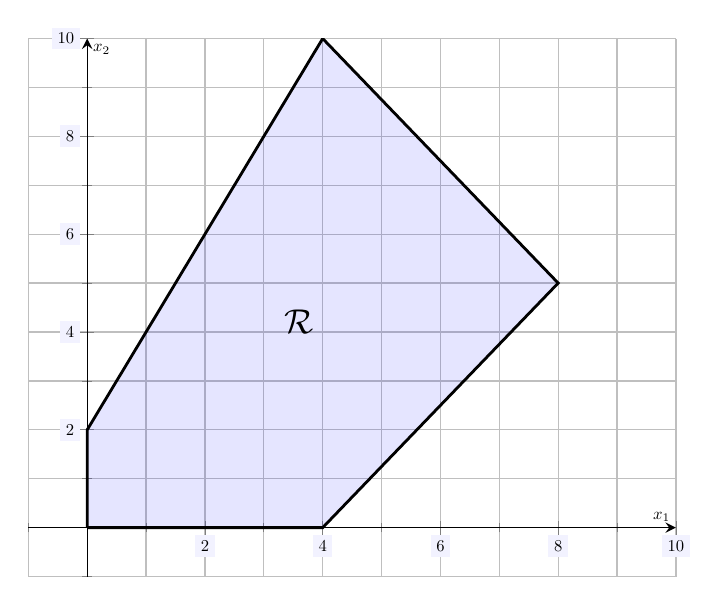
\begin{tikzpicture}[scale=1.2,every node/.style={scale=0.5}]
	\begin{axis}[
	grid=both,
	axis lines=middle,
	ticklabel style={fill=blue!5!white},
	xmin= -1, xmax=10,
	ymin= -1, ymax=10,
	xtick={0,2,4,6,8,10},
	ytick={0,2,4,6,8,10},
	minor tick = {-1,0,1,...,10},
	xlabel=\(x_1\),ylabel=\(x_2\),
	]
	\draw[line width=0.01cm,fill= blue,opacity=0.1] (0,0) -- (0,2) -- (4,10) -- (8,5) -- (4,0) -- (0,0);	
	\draw[line width=0.03cm] (0,0) -- (0,2) -- (4,10) -- (8,5) -- (4,0) -- (0,0);
	\node at (3.6,4.2) {\huge$\mathcal{R}$};
	\end{axis}
	\end{tikzpicture}
	}
	\] \pspace

\sol The function $z= x_1 + 7x_2$ is a linear function. The region $\mathcal{R}$ is a nonempty, bounded region. Therefore, by the Fundamental Theorem of Linear Programming, there exists a maximum and minimum for $z$ on $\mathcal{R}$ and they occur at a corner point for $\mathcal{R}$. We need only examine $z$ at these points: \par
	\begin{table}[h]
	\centering
	\begin{tabular}{cl}
	Corner Point & $z(x_1, x_2)$ \\ \hline
	$(0, 0)$ & $z(0, 0)= 0 + 7(0)= 0 + 0= 0$ \\
	$(0, 2)$ & $z(0, 2)= 0 + 7(2)= 0 + 14= 14$ \\
	$(4, 10)$ & $z(4, 10)= 4 + 7(10)= 4 + 70= 74$ \\
	$(8, 5)$ & $z(8, 5)= 8 + 7(5)= 8 + 35= 43$ \\
	$(4, 0)$ & $z(4, 0)= 4 + 7(0)= 4 + 0= 4$
	\end{tabular}
	\end{table} \par
Therefore, the maximum value for $z$ is $74$ and occurs at $(4, 10)$ and the minimum value for $z$ is $0$ and occurs at $(0, 0)$. 



\newpage



% Problem 4
\problem{10} Find the dual problem for the minimization problem shown below.
	\[
	\begin{gathered}
	\min w= y_1 - y_2 + y_3 \\
	\begin{cases}
	2y_1 - y_2 + y_3 \leq 9 \\
	y_1 + 5y_2 - y_3 \geq 5 \\
	3y_1 + 4y_2 + 6y_3 \geq 10 \\
	-y_1 + y_2 + 8y_3 \leq 5 \\
	y_1, y_2, y_3 \geq 0
	\end{cases}
	\end{gathered}
	\] \pspace

\sol First, we need every inequality to be of the form `$\geq$' a number. We multiply both sides of the first and fourth inequality by $-1$ to place this inequality in this form. This gives us the following inequalities (ignoring the non-negativity inequalities):
	\[
	\begin{gathered}
	\begin{cases}
	-2y_1 + y_2 - y_3 \geq -9 \\
	y_1 + 5y_2 - y_3 \geq 5 \\
	3y_1 + 4y_2 + 6y_3 \geq 10 \\
	y_1 - y_2 - 8y_3 \geq -5 
	\end{cases}
	\end{gathered}
	\]
We then form a matrix $M$ from these inequalities with the function $w= y_1 - y_2 + y_3$ as the bottom row. This gives us the following matrix: 
	\[
	M=
	\begin{pmatrix}
	-2 & 1 & -1 & -9 \\
	1 & 5 & -1 & 5 \\
	3 & 4 & 6 & 10 \\
	1 & -1 & -8 & -5 \\
	1 & -1 & 1 & 0 
	\end{pmatrix}
	\]
We then compute the transpose of this matrix:
	\[
	M^T= 
	\begin{pmatrix}
	-2 & 1 & 3 & 1 & 1 \\
	1 & 5 & 4 & -1 & -1 \\
	-1 & -1 & 6 & -8 & 1 \\
	-9 & 5 & 10 & -5 & 0 
	\end{pmatrix}
	\]
This is the `matrix of coefficients' for the inequalities for the corresponding dual maximization problem---the bottom row representing the function. The dual problem is a maximization problem so that the inequalities are `$\leq$.' Because there are $4$ columns, there are $5 - 1= 4$~variables in this system. [The last column corresponds to the `opposite' side of the inequalities.] Therefore, the dual maximization problem is\dots
	\[
	\begin{gathered}
	\max z= -9x_1 + 5x_2 + 10x_3 - 5x_4 \\
	\begin{cases}
	-2x_1 + x_2 + 3x_3 + x_4 \leq 1 \\
	x_1 + 5x_2 + 4x_3 - x_4 \leq -1 \\
	-x_1 - x_2 + 6x_3 - 8x_4 \leq 1 \\
	x_1, x_2, x_3, x_4 \geq 0
	\end{cases}
	\end{gathered}
	\] 


\end{document}